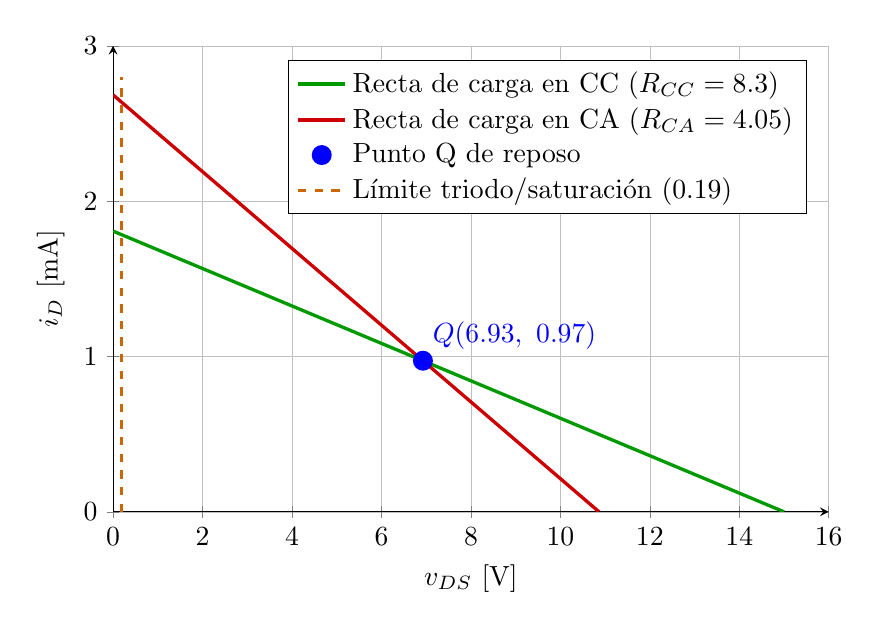
\begin{tikzpicture}
  \begin{axis}[
    width=0.88\textwidth,
    height=7.5cm,
    xlabel={$v_{DS}\ [\mathrm{V}]$},
    ylabel={$i_D\ [\mathrm{mA}]$},
    xmin=0, xmax=16.0,
    ymin=0, ymax=3.0,
    grid=both,
    grid style={line width=.1pt, draw=gray!30},
    major grid style={line width=.2pt, draw=gray!50},
    axis lines=left,
    legend pos=north east,
    legend cell align={left},
    every axis plot/.append style={very thick}
  ]
    % Recta de carga estatica (CC): i_D = (15 - x) / 8.3
    \addplot[domain=0:15.0, color=green!60!black, samples=2] {(15.0 - x) / 8.3};
    \addlegendentry{Recta de carga en CC ($R_{CC} = 8.3\kohm$)}

    % Recta de carga dinamica (CA): i_D = 0.9727 + (6.927 - x) / 4.048
    \addplot[domain=0:10.864, color=red!80!black, samples=2] {0.9727 + (6.927 - x) / 4.048};
    \addlegendentry{Recta de carga en CA ($R_{CA} = 4.05\kohm$)}

    % Punto Q de reposo
    \addplot[only marks, mark=*, mark size=3pt, color=blue] coordinates {(6.927, 0.9727)};
    \addlegendentry{Punto Q de reposo}

    % Limite de zona de saturacion (VDS = VGS - Vth = 0.190 V)
    \addplot[dashed, color=orange!80!black, samples=2] coordinates {(0.190, 0) (0.190, 2.8)};
    \addlegendentry{Límite triodo/saturación ($0.19\V$)}

    % Anotaciones
    \node[above right, text=blue] at (axis cs:6.93, 0.98) {$Q(6.93\V,\ 0.97\mA)$};
  \end{axis}
\end{tikzpicture}
